%%%%%%%%%%%%%%%%%%%%%%%%%%%%%%%%%%%%%%%%%%%%%%%%%%%%%%%%%%%%%%%%%%%%%%%%%%%%
%% Trim Size : 11in x 8.5in
%% Text Area : 9.6in (include Runningheads) x 7in
%% ws-jai.tex, 26 April 2012
%% Tex file to use with ws-jai.cls written in Latex2E.
%% The content, structure, format and layout of this style file is the
%% property of World Scientific Publishing Co. Pte. Ltd.
%%%%%%%%%%%%%%%%%%%%%%%%%%%%%%%%%%%%%%%%%%%%%%%%%%%%%%%%%%%%%%%%%%%%%%%%%%%%
%%

%\documentclass[draft]{ws-jai}
\documentclass{ws-jai}
\usepackage[flushleft]{threeparttable}
\usepackage{siunitx}
\usepackage{amsmath}
\usepackage{gensymb}
\usepackage[colorlinks=true,allcolors=blue]{hyperref}
\usepackage{graphicx}
\usepackage{caption}
\usepackage{subcaption}
\usepackage[bottom]{footmisc}
\usepackage{url}
\usepackage{natbib}


% Define stuff here
\def\albatros{ALBATROS}
\def\prizm{PRI$^{\rm Z}$M}
\newcommand{\attention}[1]{\textcolor{red}{\bf {#1}}}

\newcommand{\aap}{Astronomy and Astrophysics}
\newcommand{\aaps}{Astronomy and Astrophysics Supplements}
\newcommand{\aj}{Astronomical Journal}
\newcommand{\apj}{Astrophysical Journal}
\newcommand{\grl}{Geophysical Research Letters}
\newcommand{\jgr}{Journal of Geophysical Research}
\newcommand{\mnras}{Monthly Notices of the Royal Astronomical Society}
\newcommand{\nar}{New Astronomy Reviews}
\newcommand{\pasa}{Publications of the Astronomical Society of Australia}
\newcommand{\pasp}{Proceedings of the Astronomical Society of the Pacific}
\newcommand{\prd}{Physical Review D}
\newcommand{\prl}{Physical Review Letters}

\begin{document}

\catchline{}{}{}{}{} % Publisher's Area please ignore

\markboth{Author's Name}{ALBATROS instrument}

\title{The Array of Long-Baseline Antennas for Taking Radio
  Observations from the Sub-Antarctic}

\author{First Author$^{2}$, Second Author$^{3}$, Third Author$^{3}$ and Fourth Author$^{4}$}

\address{
$^{2}$Department, University Name, City, State ZIP/Zone, Country, fauthor@university.com\\
$^{3}$Group, Company, Address, City, State ZIP/Zone, Country\\
$^{4}$Group, Company, Address, City, State ZIP/Zone, Country, fauthor@company.com
}

\maketitle

\corres{$^{2}$Corresponding author.}

\begin{history}
\received{(to be inserted by publisher)};
\revised{(to be inserted by publisher)};
\accepted{(to be inserted by publisher)};
\end{history}

\begin{abstract}
Measurements of redshifted 21-cm emission of neutral hydrogen at
$\lesssim30$~MHz have the potential to probe the cosmic ``dark ages,''
a period of the universe's history that remains unobserved to date.
Observations at these frequencies are exceptionally challenging
because of bright Galactic foregrounds, ionospheric contamination, and
terrestrial radio-frequency interference.  Very few sky maps exist at
$\lesssim30$~MHz, and most have modest resolution.  We introduce the
Array of Long Baseline Antennas for Taking Radio Observations from the
Sub-Antarctic (\albatros), a new experiment that aims to image
low-frequency Galactic emission with an order-of-magnitude improvement
in resolution over existing data.  The \albatros\ array will consist
of antenna stations that operate autonomously, each recording baseband
data that will be interferometrically combined offline.  The array
will be installed on Marion Island and will ultimately comprise 10
stations, with an operating frequency range of 1.2--125~MHz and
maximum baseline lengths of $\sim20$~km.  We present the
\albatros\ instrument design and discuss pathfinder observations that
were taken from Marion Island during 2018--2019.
\end{abstract}

\keywords{cosmology: observations; dark ages; instrumentation: interferometers}

\section{Introduction}

Measurements of redshifted \SI{21}{\cm} emission of neutral hydrogen
across a wide range of radio frequencies have the potential to
elucidate the universe's history from the cosmic ``dark ages'' up to
the formation of large-scale
structures~\citep[e.g.,][]{2012RPPh...75h6901P}.  The dark ages, which
occurred after recombination and correspond to a period when the
universe was filled with neutral hydrogen, are unexplored to date and
represent one of the final observational frontiers in cosmology.  The
number of independent modes that are contained in the matter power
spectrum in this epoch is orders of magnitude greater than the
corresponding number for cosmic microwave background (CMB)
measurements~\citep{2004PhRvL..92u1301L}.  Redshifted 21-cm
measurements of the dark ages therefore hold the potential to
significantly improve cosmological parameter constraints over those
currently derived from the CMB; however, the required observational
frequencies of $\lesssim 30$~MHz are exceptionally difficult to
access.  The primary experimental challenges include Galactic
foreground emission, ionospheric interference, and terrestrial
radio-frequency interference (RFI).

Very few experiments have surveyed the radio sky at $\lesssim 30$~MHz,
and here, we highlight only four specific examples.  At the very
lowest frequencies, the state of the art among ground-based
measurements dates from the 1950s, when Reber and Ellis caught brief
glimpses of the $2.1$~MHz sky at $\sim 5$\degree\ resolution, using an
array of 192~dipoles~\citep{1956JGR....61....1R}.  A few space-based
missions have also performed measurements at similarly low frequency
ranges; for example, the Radio Astronomy Explorer-2 operated at
\SIrange{0.025}{13}{\MHz} with $\sim 10$\degree\ resolution at
\SI{4.7}{\MHz}~\citep{1975A&A....40..365A}.  Measurements with
resolution finer than few-degree scales exist mainly at higher
frequencies.  For example, the Dominion Radio Astrophysical
Observatory surveyed the northern sky at \SI{22}{\MHz} with
\SIrange{1.1}{1.7}{\degree} resolution~\citep{1999A&AS..137....7R},
and most recently, the Owens Valley Long Wavelength Array mapped the
sky with \SI{15}{\arcminute} resolution between 36.528~MHz and
73.152~MHz~\citep{2018AJ....156...32E}.  Although this experimental
list is not comprehensive, it does illustrate the dearth of
information about the $\lesssim 30$~MHz sky and the lack of high
resolution measurements at the lowest frequencies.  The first step
toward laying the groundwork for possible measurements of the dark
ages is obtaining an improved map of Galactic foregrounds at $\lesssim
30$~MHz.  In addition to serving as a stepping stone for future
cosmological constraints from the dark ages, maps at these frequencies
can also shed new light on Galactic astrophysics.  Above $\sim30$~MHz,
synchrotron emission from the Galaxy follows a power law with a
frequency dependence of $\sim \nu^{-0.7}$.  At lower frequencies,
synchrotron self-absorption becomes non-negligible, and the spectrum
transitions to $\nu^{+5/2}$ dependence.  Since self-absorption causes
the optical depth along the line of sight to depend on frequency,
observations at $\lesssim 30$~MHz have the potential to probe the
three-dimensional cosmic ray structure of the
Galaxy~\citep{2002ApJ...575..217P}.  Low-frequency observations can
also be used to image radio recombination lines (RRLs), which provide
a means for studying cool, low-density regions of the interstellar
medium (ISM).  These absorption lines arise from Rydberg atoms and are
highly sensitive to the surrounding environment.  The RRL spectrum and
absorption profiles can therefore constrain the detailed properties of
the ISM regions in which the Rydberg atoms are
formed~\citep{2009NewAR..53..259G, 2007MNRAS.374..852S}.  Finally,
observations at $\lesssim30$~MHz may provide new views of Earth's
ionosphere, which absorbs and refracts at radio frequencies and
becomes completely opaque below the plasma cutoff frequency.  The
cutoff frequency and the levels of absorption and refraction are
time-varying and spatially dependent.  Experiments that image the
radio sky at multiple frequencies bracketing the plasma cutoff can
therefore simultaneously image the ionosphere and provide spectral
riometry data for space weather studies~\citep{2014GeoRL..41.5370K}.

\begin{figure}
  \begin{center}
    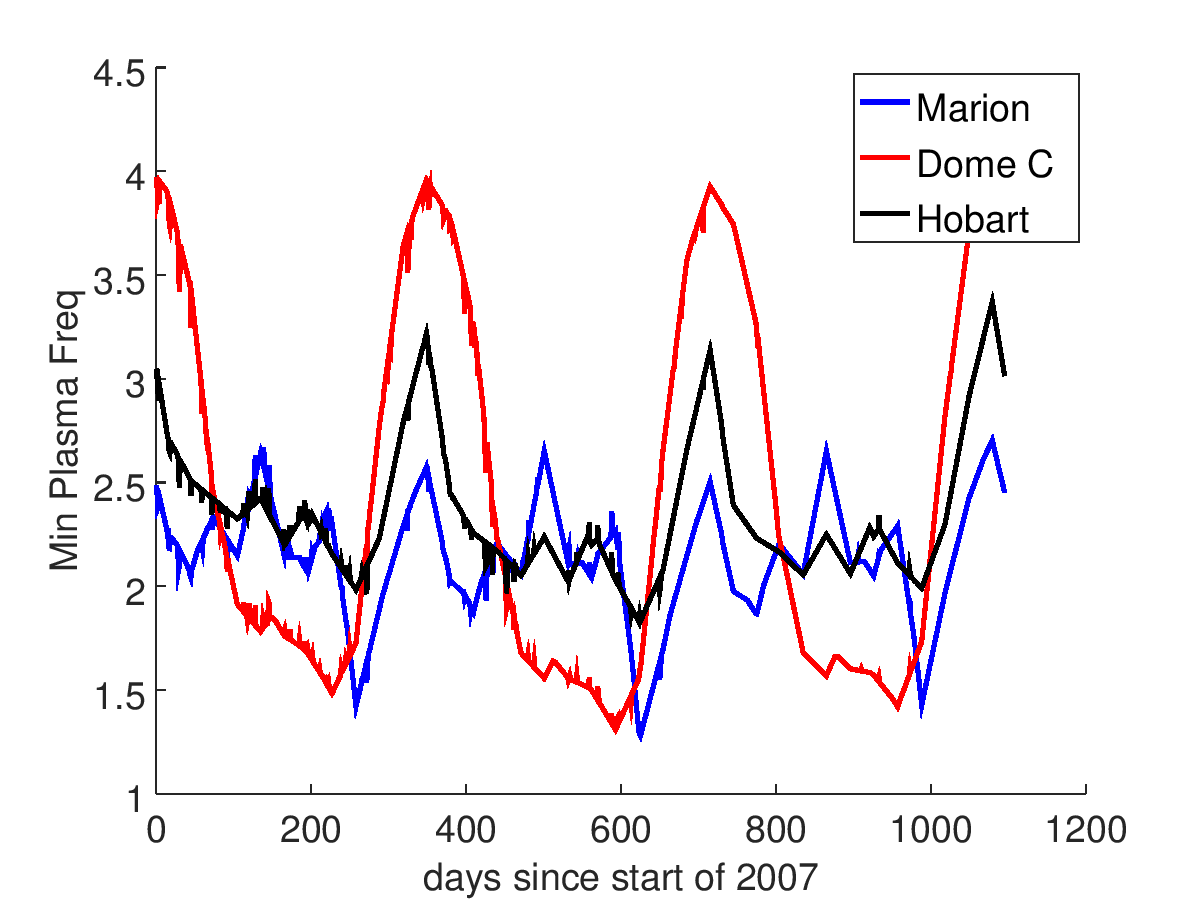
\includegraphics[width=0.6\linewidth]{Figures/marion_domec_hobart.png}
    \caption{Minimum plasma frequency predicted by the International
      Reference Ionosphere model during the last solar minimum.  At
      some locations on Earth, the plasma frequency may drop as low as
      $\sim1.5$~MHz.}
    \label{Fig:iri}
  \end{center}
\end{figure}

There are proposed efforts to perform new low-frequency measurements
from space, where there is no contamination from the ionosphere, and
the lunar farside can potentially block RFI from the
Earth~\citep{2019arXiv190710853C, 2019arXiv190804296K}.  Although the
combination of ionosphere and RFI significantly impedes low-frequency
radio observations from most locations on Earth, preliminary
observations from Marion Island~\citep{2019JAI.....850004P} suggest
that such observations may still be accessible from carefully selected
locations and with new technology developments.  In this paper, we
present the Array of Long Baseline Antennas for Taking Radio
Observations from the Sub-Antarctic (\albatros), a new experimental
effort that aims to map the low-frequency sky using an array of
autonomous antenna stations.  We describe the overall instrument
design and preliminary measurements from engineering runs that were
performed on Marion Island during 2018--2019.

\begin{figure}
    \centering
    \begin{subfigure}[t]{0.6\textwidth}
        \centering
        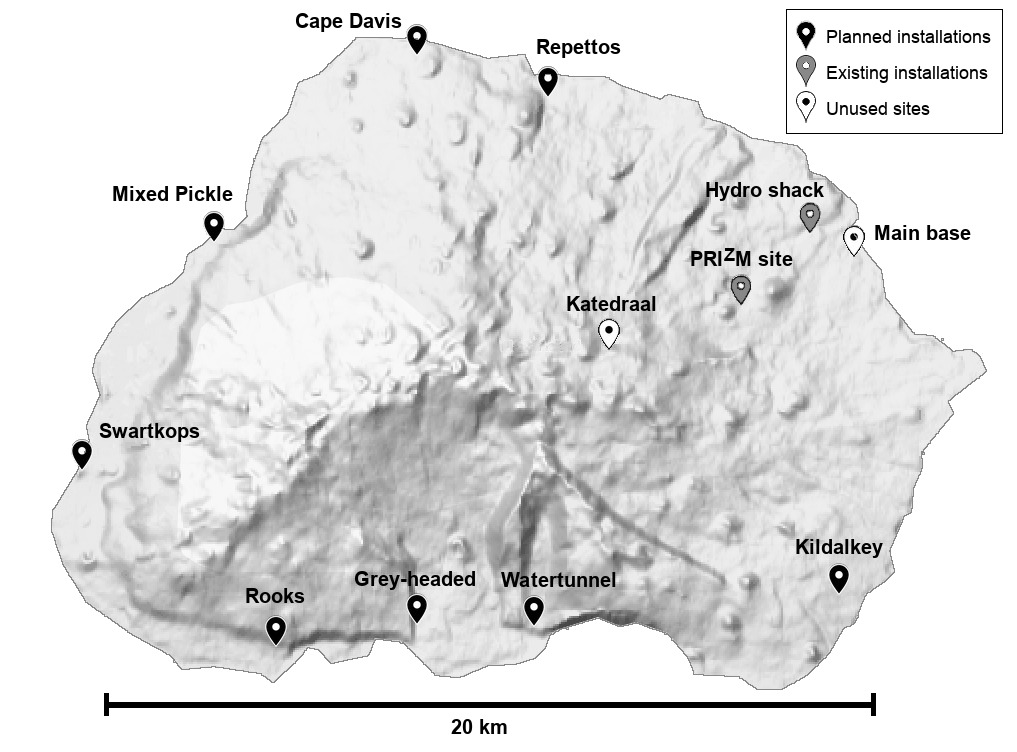
\includegraphics[width=\linewidth]{Figures/marion_map/marion_map_annotated.jpg} 
        \caption{} \label{Fig:marion_map}
    \end{subfigure}
    \hfill
    \begin{subfigure}[t]{0.39\textwidth}
      \centering
        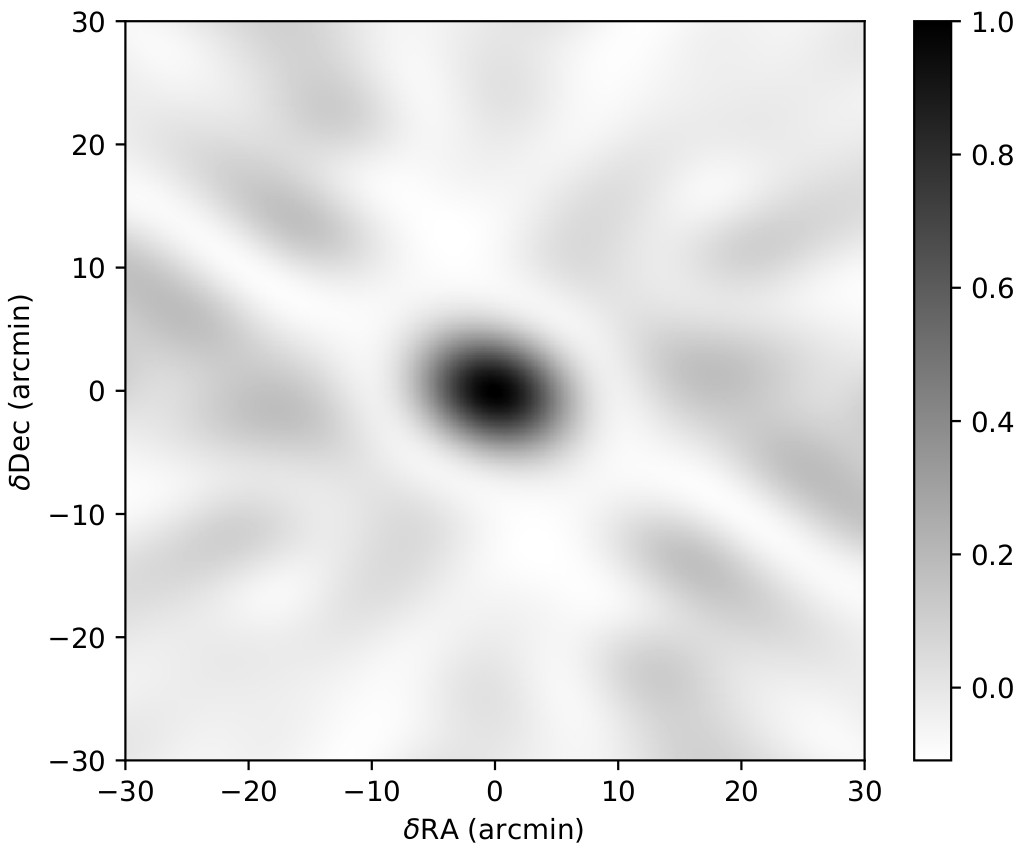
\includegraphics[width=\linewidth]{Figures/marion_beam_huts_2020.jpg}
        \caption{} \label{Fig:marion_beam}
    \end{subfigure}
    \caption{{\bf (a)} Map of Marion Island.  The
      \albatros\ pathfinder antennas are currently installed at the
      \prizm\ site and at the hydro shack (gray markers).  The black
      markers denote the eight coastal huts, which will be used for
      future \albatros\ antenna installations.  The white markers
      denote other available infrastructure points that will not be
      used for antennas.  {\bf (b)} Synthesized beam at 5~MHz at zenith from the
      full \albatros\ array, using the existing and planned
      installation locations shown on the map.  Using an octave of
      bandwidth spanning 3.5--7~MHz in a single snapshot, we obtain a synthesized beam with 
      a full width of $\sim7'$.}\label{Fig:marion_map_beam}
\end{figure}

\section{ALBATROS overview}

The primary requirements that drive the design for a low-frequency
imaging experiment are 1) desired resolution, 2) low RFI, and 3) quiet
ionospheric conditions.  As a benchmark, an interferometer operating
at 30~MHz requires baseline lengths of $\sim0.5$--1~km 
to achieve a resolution of $\sim 1$\degree.  This length scales
inversely with frequency, and therefore $\sim 10$-km lengths are
required at few-MHz frequencies to improve substantially upon the resolutions
achieved to date.  The experiment installation site must be remote to
keep RFI to a minimum, and polar or near-polar latitiudes generally
have lower ionospheric plasma frequency cutoffs relative to other
locations on Earth.  \autoref{Fig:iri} illustrates predictions from
the International Reference Ionosphere
model~\citep{2018AdRS...16....1B} for the minimum plasma frequency
during the last solar minimum, which started in approximately 2007.
Three locations are shown: Marion Island, the focus of this work;
Dome~C in Antarctica, which is another isolated location used for
astronomical observations; and Hobart, Tasmania, where Reber performed
his $\sim2$~MHz observations.  The model predictions illustrate that
the ionospheric plasma cutoff frequency at Marion Island may drop as
low as $\sim1.5$~MHz during solar minima.  Since we are currently
experiencing another solar minimum~\citep{2018NatCo...9.5209B}, the
timing is opportune for new low-frequency observations.

Marion Island is a research base that is located in the southern
Indian Ocean at \ang{46;54;45}S, \ang{37;44;37}E and is operated by
the South African National Antarctic Programme.  The island lies
roughly \SI{2000}{\kilo\metre} from the nearest continental landmasses
and has an exceptionally quiet RFI
environment~\citep{2019JAI.....850004P}.  As illustrated in
\autoref{Fig:marion_map}, Marion has an area of 335~km$^2$ and can
therefore support antenna installations with $>10$-km baseline
lengths.  The main Marion base is located on the northeast side of the
island, and there are eight rest huts along the coast (Cape Davis,
Grey-headed, Kildalkey, Mixed Pickle, Repettos, Rooks, Swartkops,
Watertunnel) and one in the interior (Katedraal) that can serve as
existing infrastructure points for antenna installations.  The planned
\albatros\ installation sites include the coastal huts, but exclude
the main base and Katedraal for RFI and accessibility reasons,
respectively.  \autoref{Fig:marion_map} also shows the locations of
the \albatros\ pathfinder antennas that are currently installed at the
\prizm\ site and at the hydro shack.

Using the eight coastal huts, the \prizm\ site, and the hydro shack as
the nominal \albatros\ installation locations, the computed
synthesized beam is as shown in \autoref{Fig:marion_beam}.  The beam
width at 5~MHz is roughly \SI{7}{\arcminute}, which represents over an
order of magnitude improvement in resolution over other existing
measurements.  One of the challenges in constructing an interferometer
array on Marion Island is that the rugged terrain precludes the
possibility of directly cabling and correlating antennas across large
distances.  The final \albatros\ antenna stations will therefore
operate {\it autonomously}, recording baseband data over extended
periods of time for subsequent offline correlation.  We have conducted
two engineering runs: 1) a two-element, directly correlated pathfinder
to qualitatively understand the sky signal, and 2) a single station to
test the readout and power handling technology that are required for
autonomous operation.

\section{Two-element pathfinder}\label{s:2elem}

\begin{figure}
  \begin{center}
    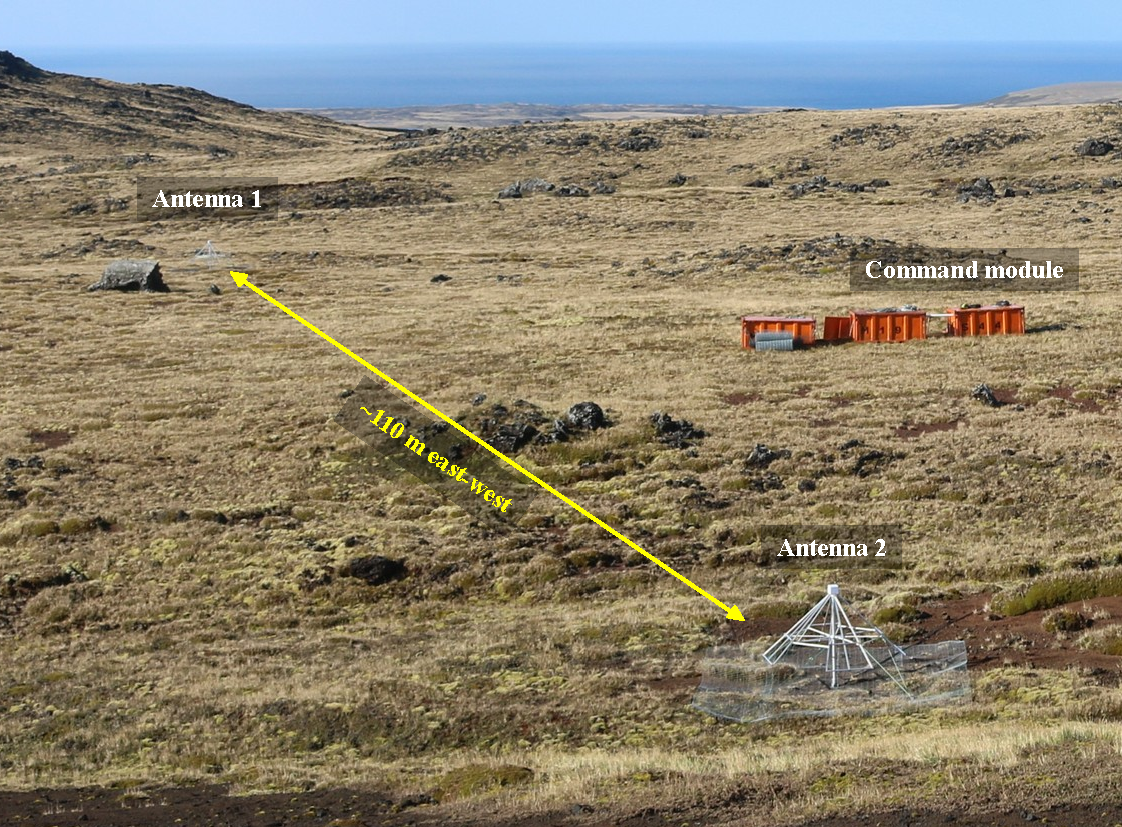
\includegraphics[width=0.7\linewidth]{Figures/albatros_2elem/albatros_2elem.pdf}
    \caption{The two-element, directly correlated
      \albatros\ pathfinder installed at the \prizm\ site.  Two
      dual-polarization antennas are separated by roughly 110~m on an
      east--west baseline. Coaxial cables connect the antennas to a
      shipping container that houses the readout electronics and
      serves as the ``command module.''}
    \label{Fig:albatros2}
  \end{center}
\end{figure}

\begin{figure}
  \begin{center} 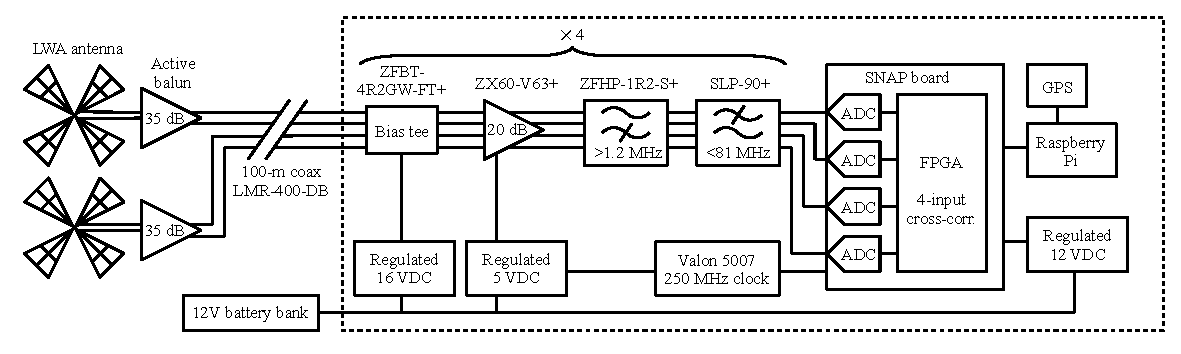
\includegraphics[width=1.0\linewidth]{Figures/albatros_2elem_schematic/albatros_2elem_schematic.pdf}
    \caption{Two-element \albatros\ pathfinder block diagram.  Signals
      from two dual-polarization LWA antennas are amplified by
      front-end active baluns~\citep{2012PASP..124.1090H}.  The
      antennas are connected via 100-m coaxial cables to the back-end
      readout electronics, which are housed in a Faraday cage denoted
      by the dashed box.  Each of the four antenna outputs is passed
      to a second-stage electronics chain consisting of filters and
      further amplfication.  The signals are digitized at 250~Msamp/s
      by a SNAP board, which includes an on-board FPGA that computes
      auto- and cross-spectra from and between the four inputs.  A
      Raspberry Pi controls the SNAP board and saves the data.}
    \label{Fig:albatros2_schem}
  \end{center}
\end{figure}

The first exploratory \albatros\ measurements were conducted with a
two-element pathfinder that used direct correlation (without
autonomous operation).  \autoref{Fig:albatros2} illustrates this
pathfinder, which was installed at the \prizm\ site (\ang{46;53;13}S,
\ang{37;49;10.7}E) in April 2018.  The system block diagram is shown
in \autoref{Fig:albatros2_schem}, and each of the subsystems is
described in detail below.

\subsection{Antenna}\label{s:antenna}

We employ two dual-polarization Long Wavelength Array (LWA) dipole
antennas~\citep{Memo28}.  The LWA antennas have a long development
history, are well characterized, and are simple to install and
physically robust.  The antennas form an east--west baseline with a
separation of \SI{110}{m}, and the polarizations are aligned with the
cardinal directions.  Welded wire mesh screens, roughly 3~m on a side,
are installed on the ground below the antennas.  Although the LWA
antenna is not optimized for observations below 10~MHz, using this
standard antenna allowed an initial test of the site and of the
interferometer systems.  For the final \albatros\ array, we are
exploring alternative antenna designs that will cover the full
frequency range.

% do we want/need to say anything about the omnidirectional primary beam?

\subsection{Front-end active balun}\label{s:fee}

The LWA active-balun front-end electronics (FEE) circuit uses a
MiniCircuits GALI-74+ MMIC to amplify each dipole leg against ground,
presenting each leg with a 50$\ohm$ impedance and providing a nominal
gain of 25~dB. The two GALI-74+ outputs are differenced using a
passive {180\degree} hybrid coupler. The coupler output is filtered by
a $\sim$150~MHz lowpass and receives an additional 12~dB of gain from
a MiniCircuits GALI-6+ MMIC. This last amplifier drives the output
signal onto a 100-m 50$\ohm$ coaxial cable. Thus, neglecting mismatch
loss between the dipoles (electrically small in the frequency range of
interest) and the 100{\ohm} input impedance, as well as the hybrid
insertion loss ($<$1dB), the front-end electronics provide a gain of
$\sim$37~dB~\citep{2012PASP..124.1090H}.  Each FEE circuit is powered
by 16~V, which is fed on the coaxial cable through a bias tee.

% EE citing the noise figure of the GALI-74+ is particulary misleading because of the large mismatch loss, which directly scales up the noise figure in the HF band. 

%% It seems to me that this is too much detail to go into in describing an already published design.
% All the front end components were incorporated for in a double sided
% printed circuit board (PCB) as shown in \autoref{Fig:Balun} and the
% block diagram is shown in \autoref{Fig:Balun Schematic}. The
% Monolithic Microwave Integrated Circuits (MMICs) is the used design
% for the PCB. One side of the PCB is populated with components and
% the other side is a solid copper ground plane aperiodically stitched
% to the grounded copper on the side populated with components. The
% receiver system is made up of the active balun, filter and the gain
% stage that connects to the \SI{100}{\metre} coaxial cable which is
% connected to the back end \cite{2012PASP..124.1090H}.

% The input impedance (Z\textsubscript{o}) of \SI{50}{\ohm} is
% introduced to the dipole by the active balun. The signal is then fed
% through an amplifier which amplifies it by \SI{+24}{\decibel} of
% gain. The balanced signal is then converted to unbalanced through a
% 180 \degree hybrid coupler. The band pass filter (BPF) receives the
% single ended signal in order for it to reject all the frequencies
% which are not within the range of interest. The signal gets fed to a
% second amplifier which again amplies it by \SI{+24}{\decibel} of gain
% and the output impedance of the FEE is matched to a \SI{50}{\ohm}
% coaxial cable. The bias tee is responsible for providing power to the
% FEE and extracts the RF signal by the use of the coaxial cable. This
% unit has an overall gain of $\approx$ \SI{35}{\decibel} and an overall
% noise figure of $\approx$ \SI{2.7}{\decibel} to $\approx$
% \SI{2.9}{\decibel} \cite{Memo35}.

\subsection{Back-end electronics}

The back-end readout electronics are housed in a Faraday cage located
100~m away from the antennas to mitigate possible self-generated RFI.
Each of the four antenna signals is passed to a second-stage
electronics chain consisting of an amplifier (Minicircuits ZX60-V63+),
and a pair of high- and low-pass filters (Minicircuits ZFHP-1R2+ and
SLP-90+) that together band-limit the signal to 1.2--\SI{81}{MHz}.
The amplifier has a nominal gain of 20~dB, and the high- and low-pass
filters contribute nominal insertion losses of 0.2~dB and 0.14~dB,
respectively.

A Smart Network ADC Processor~\citep[SNAP;][]{2016JAI.....541001H}
board digitizes the RF signals at 250~Msamp/s and uses a Xilinx
Kintex~7\footnote{\url{http://www.xilinx.com/products/silicon-devices/fpga/kintex-7.html}}
FPGA to calculate full cross-correlations of the four inputs,
producing four auto- and six cross-spectra as outputs, over 2048
channels spanning the frequency range 0--125~MHz.  The channelization
is performed with a
CASPER\footnote{\url{https://casper.berkeley.edu/}}-based polyphase
filter bank, and the spectra are accumulated over $\sim7$-s intervals.
A Valon 5007 frequency synthesizer module provides the clock signal
for the SNAP board.  A Raspberry Pi (RPi)~3B+ single board computer
controls the SNAP board and receives the spectra via GPIO connections.
The data rate of the averaged spectra is roughly 400~MB/day (with
compression), and this low volume allows the spectra to be saved to
the RPi on-board SD card.  An Adafruit Ultimate GPS
module\footnote{\url{https://www.adafruit.com/product/746}}, connected
to an active external GPS antenna, provides absolute timing for the
RPi.

% data rate ~ 17MB/hour, with compressed scio files

\subsection{Power}

A bank of four 12-V, 200-Ah AGM batteries, connected in parallel,
powers the two-element pathfinder system.  The batteries are manually
charged with a Honda EU30is generator that is housed on site.  The
total power draw of the two-element pathfinder is $\sim45$~W, and when
fully charged, the battery bank can power the system for about a week.
The raw battery voltage is passed to several DC/DC converters that
supply regulated voltages to the SNAP board, FEE, amplifiers and the
clock.

%%%%%%%%%%%%%%%%%%%%%%%%%%%%%%%%%%%%%%%%%%%%%%%%%%%%%%%%%%%%%5

\section{Single autonomous station pathfinder}

\begin{figure}
    \centering
    \begin{subfigure}[t]{0.48\textwidth}
        \centering
        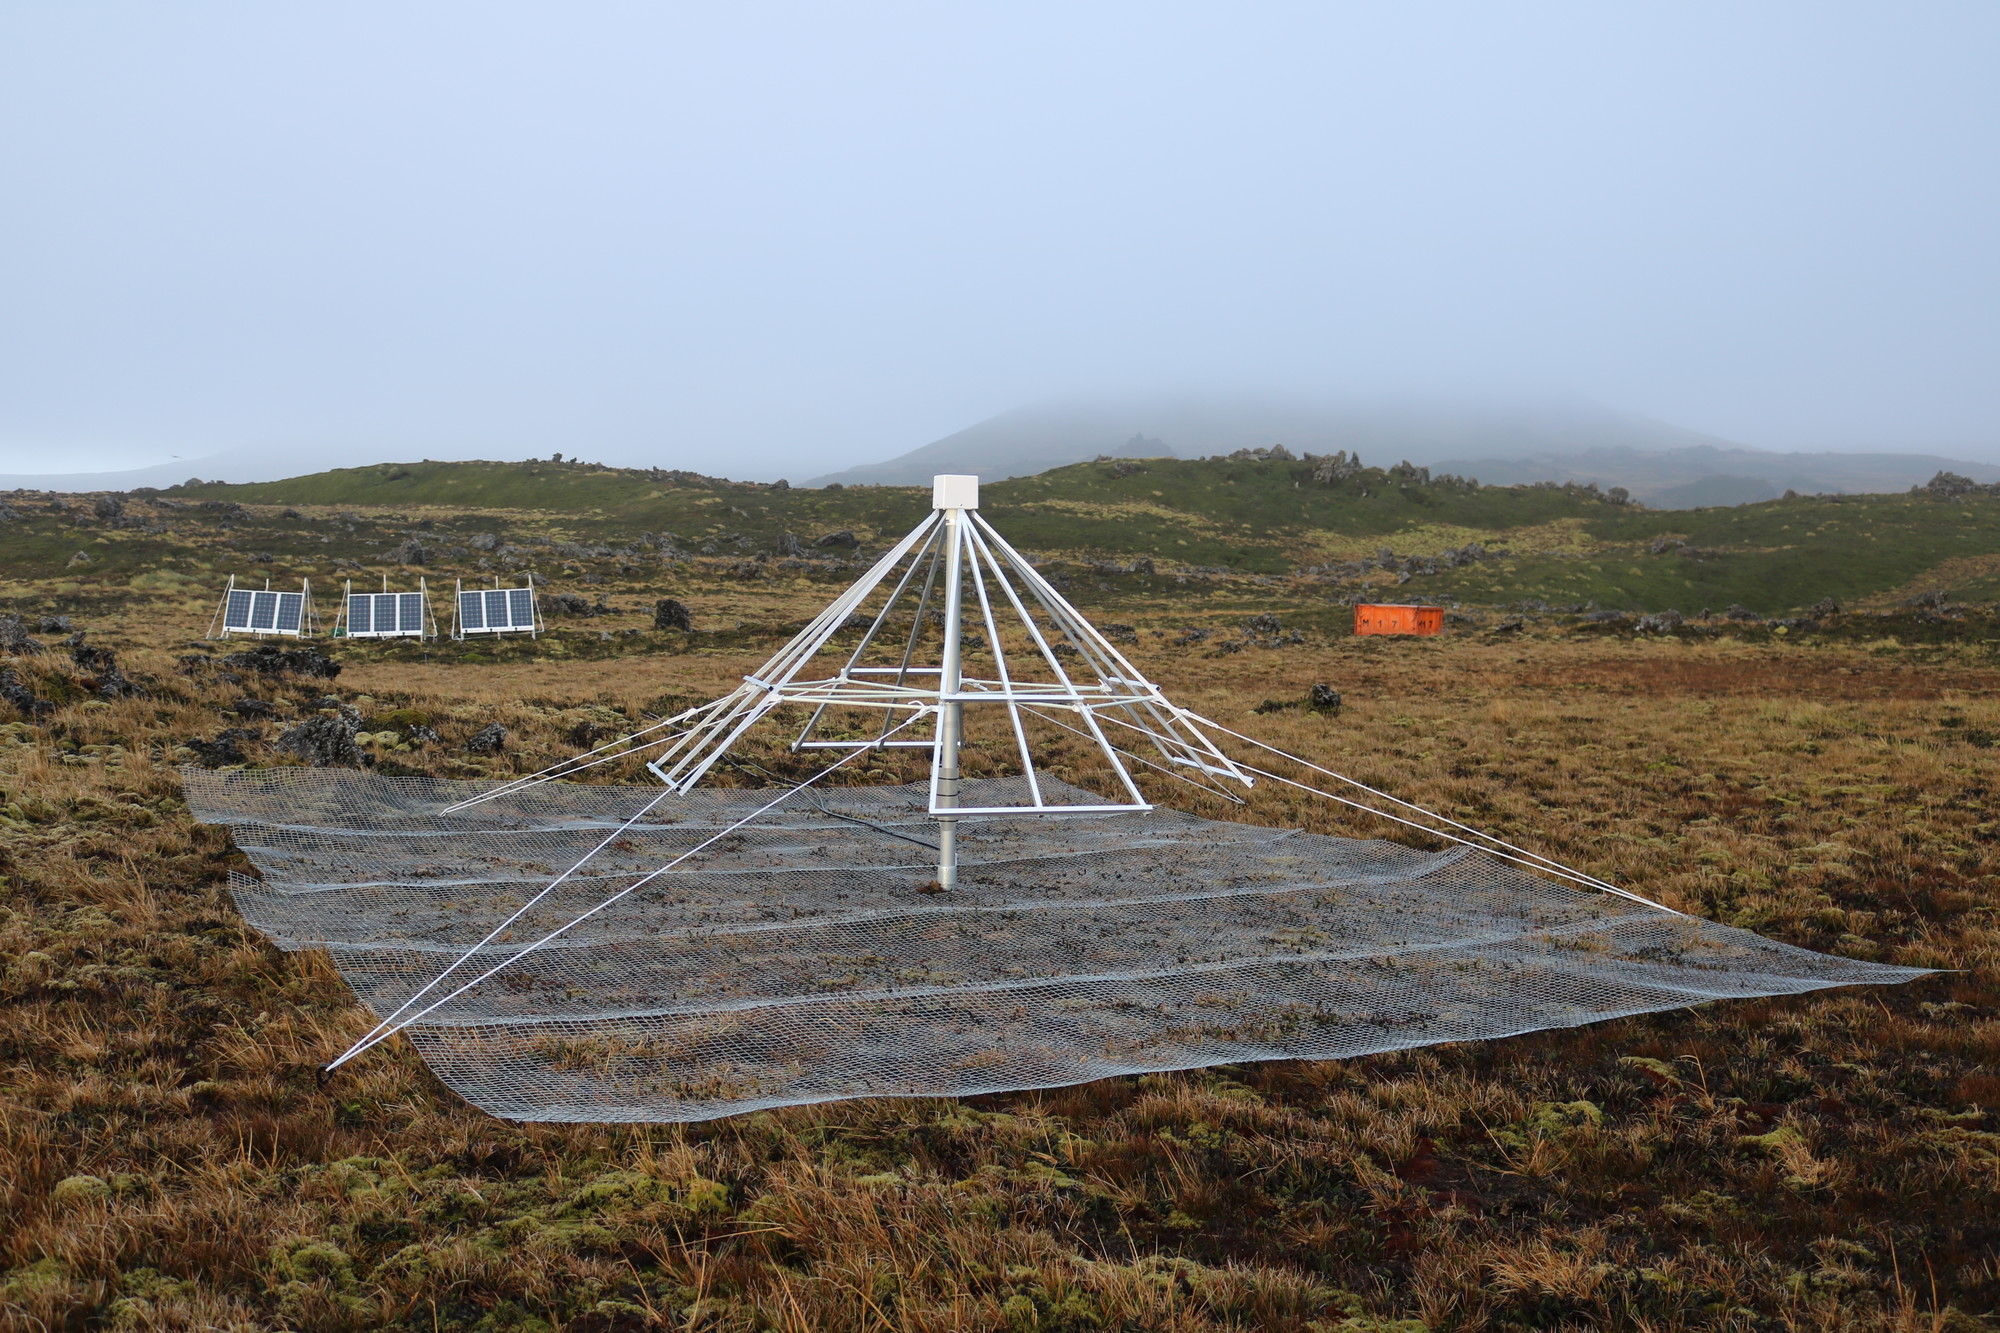
\includegraphics[width=\linewidth]{Figures/autonomous.jpg} 
        \caption{} \label{Fig:autonomous_antenna}
    \end{subfigure}
    \hfill
    \begin{subfigure}[t]{0.48\textwidth}
      \centering
        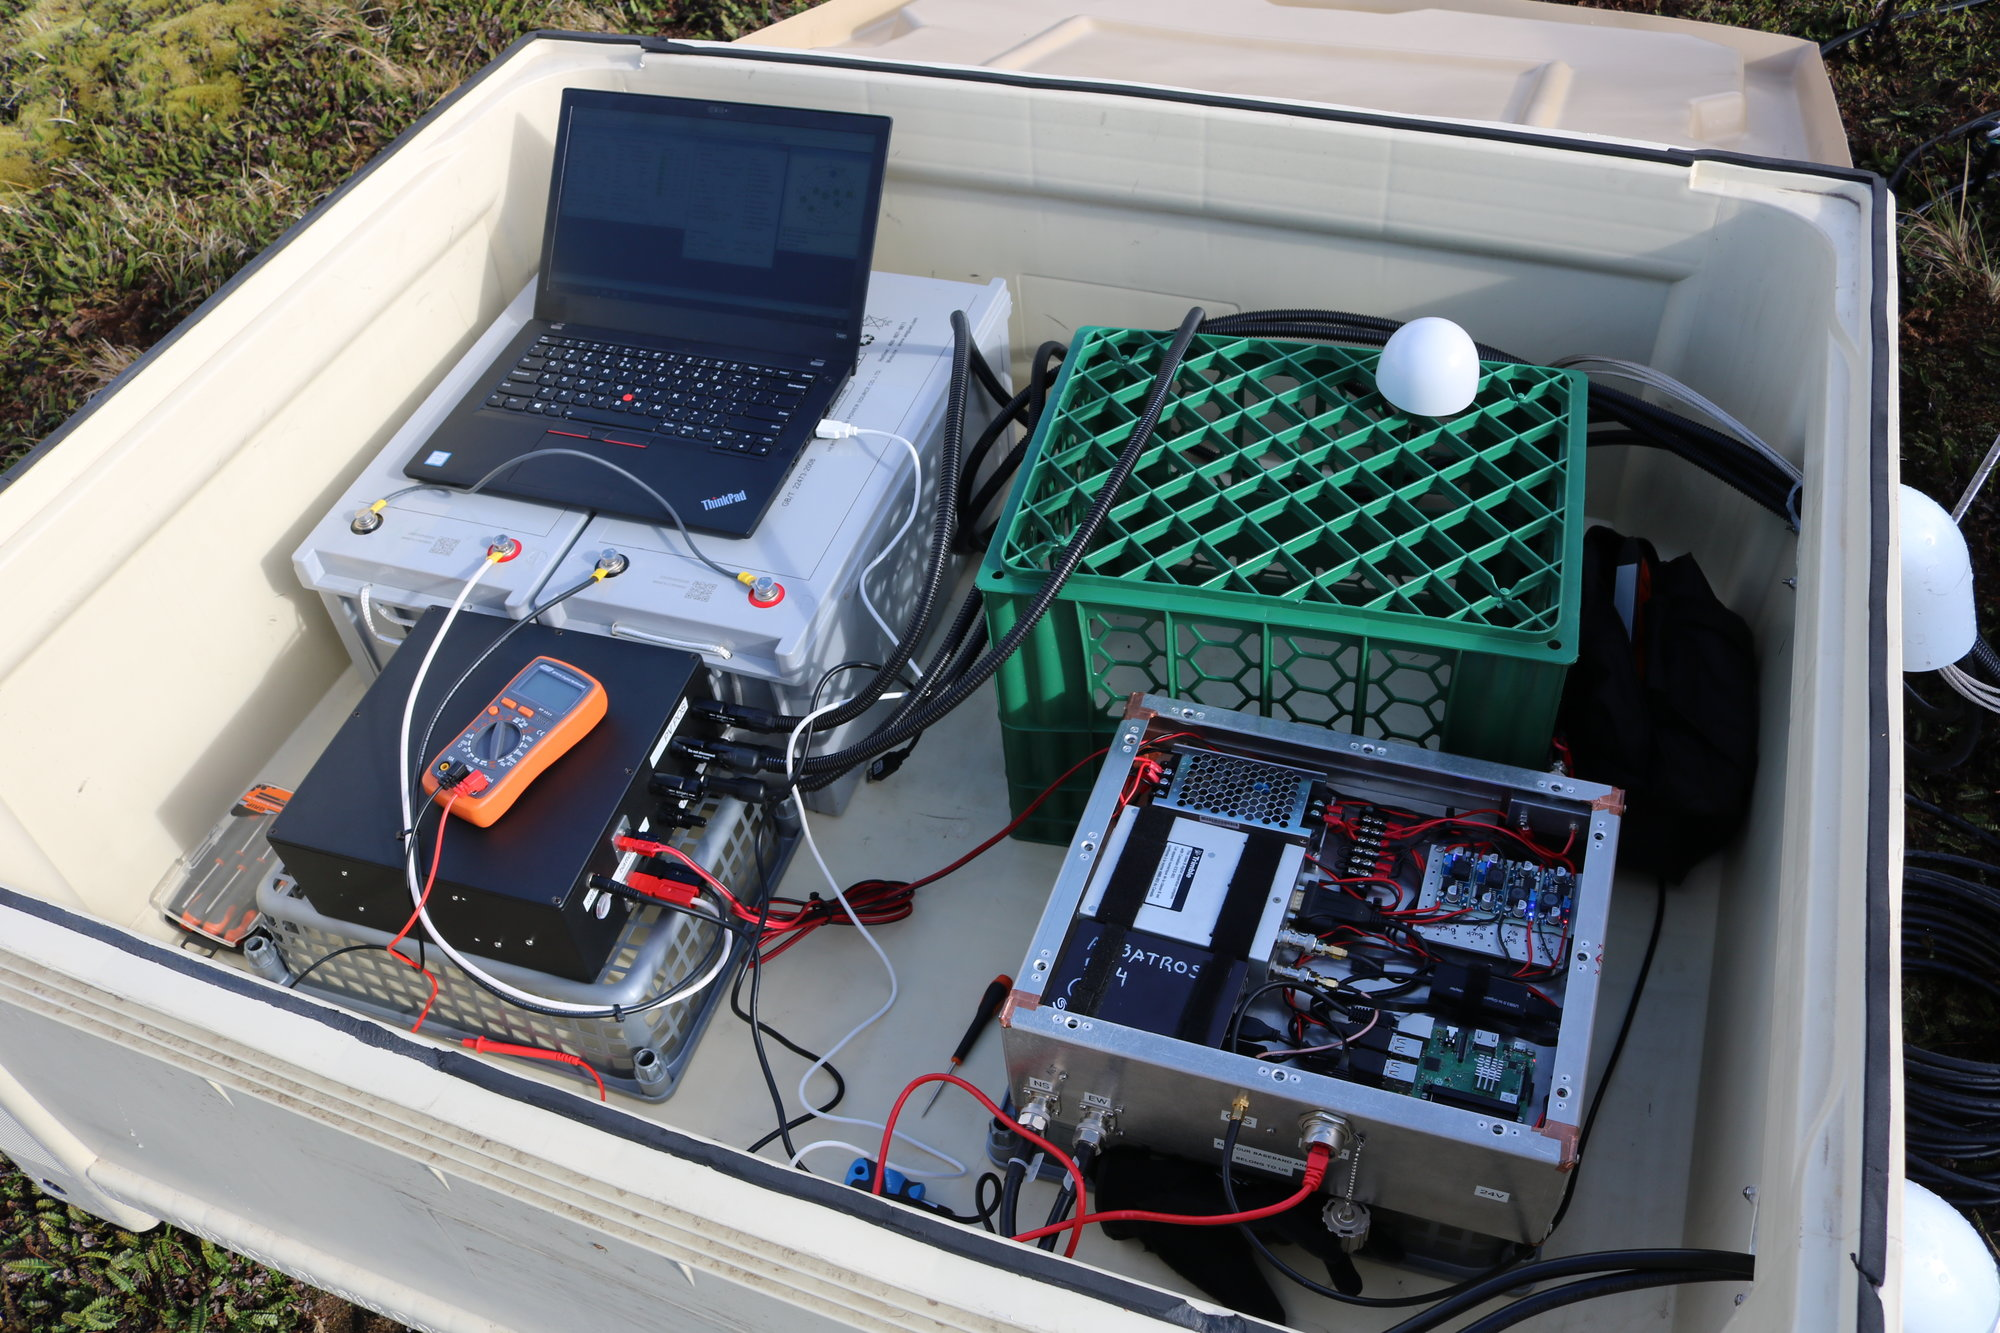
\includegraphics[width=\linewidth]{Figures/container.jpg}
        \caption{} \label{Fig:autonomous_electronics}
    \end{subfigure}
    \caption{{\bf (a)} Single autonomous station pathfinder installed
      at the hydro shack site.  The system is powered by a bank of
      solar panels that are visible in the background. {\bf (b)} A
      weather-proof container, which sits near the solar panels,
      houses the batteries, solar charge controller, and readout
      electronics.}\label{Fig:autonomous}
\end{figure}

\begin{figure}
  \begin{center}
    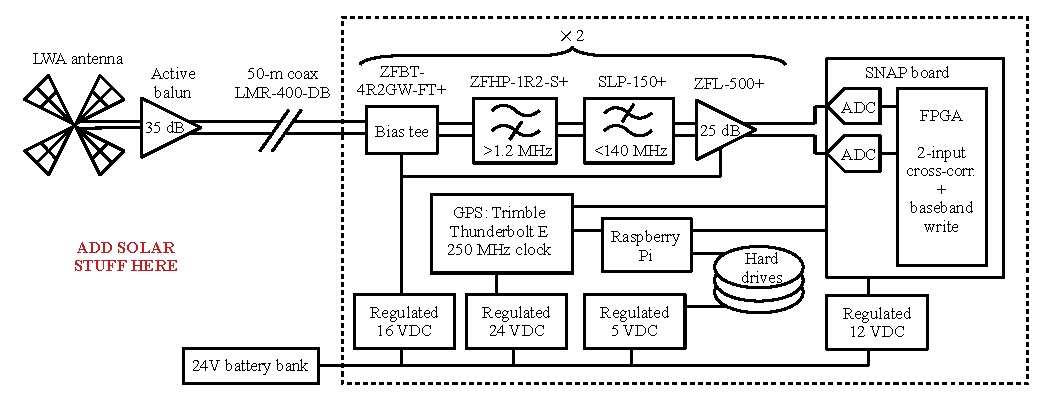
\includegraphics[width=\linewidth]{Figures/albatros_single_schematic/albatros_single_schematic.pdf}
    \caption{Single-antenna autonomous station block diagram.  A
      dual-polarization LWA antenna, equipped with a front-end active
      balun, connects via 50-m coaxial cables to the back-end readout
      electronics, housed in a Faraday cage denoted by the dashed box.
      Each of the two antenna signals is passed to a second-stage
      electronics chain consisting of filters and further
      amplfication.  The signals are digitized at 250~Msamp/s by a
      SNAP board, which includes an on-board FPGA that computes
      channelized baseband and spectra from both inputs.  A Raspberry
      Pi controls the SNAP board and receives the baseband data and
      spectra.  The baseband data are saved to external hard drives.
      The system is powered by solar panels that charge a 24-V battery
      bank.}
    \label{Fig:albatros1_schem}
  \end{center}
\end{figure}

The full \albatros\ configuration will comprise an array of 10
autonomous antenna stations, each recording baseband over tunable
frequency windows (with 10--20~MHz total bandwidth) within the full
0--125~MHz operating range.  The baseband data will be collected
periodically and subsequently correlated offline.  The
\albatros\ stations, located at the eight coastal hut sites plus the
hydro shack and \prizm\ site, will be separated by baselines of
$\sim20$~km as shown in \autoref{Fig:marion_map_beam}. One fully
autonomous \albatros\ station, shown in \autoref{Fig:autonomous}, was
deployed in April 2019 at the hydro shack location (\ang{46;52.205;}S,
\ang{37;50.612;}E) on Marion Island as a first step in testing the
technology needed to establish the full array.  The system block
diagram is shown in \autoref{Fig:albatros1_schem}.  The antenna and
front-end active balun in the single autonomous station are identical
to those used in the two-element pathfinder (\S\ref{s:antenna} and
\S\ref{s:fee}), and the back-end electronics and power system are
described in detail below.

% HCC: we probably don't need this figure
% \begin{figure}[h]
% 	\begin{center}
% 		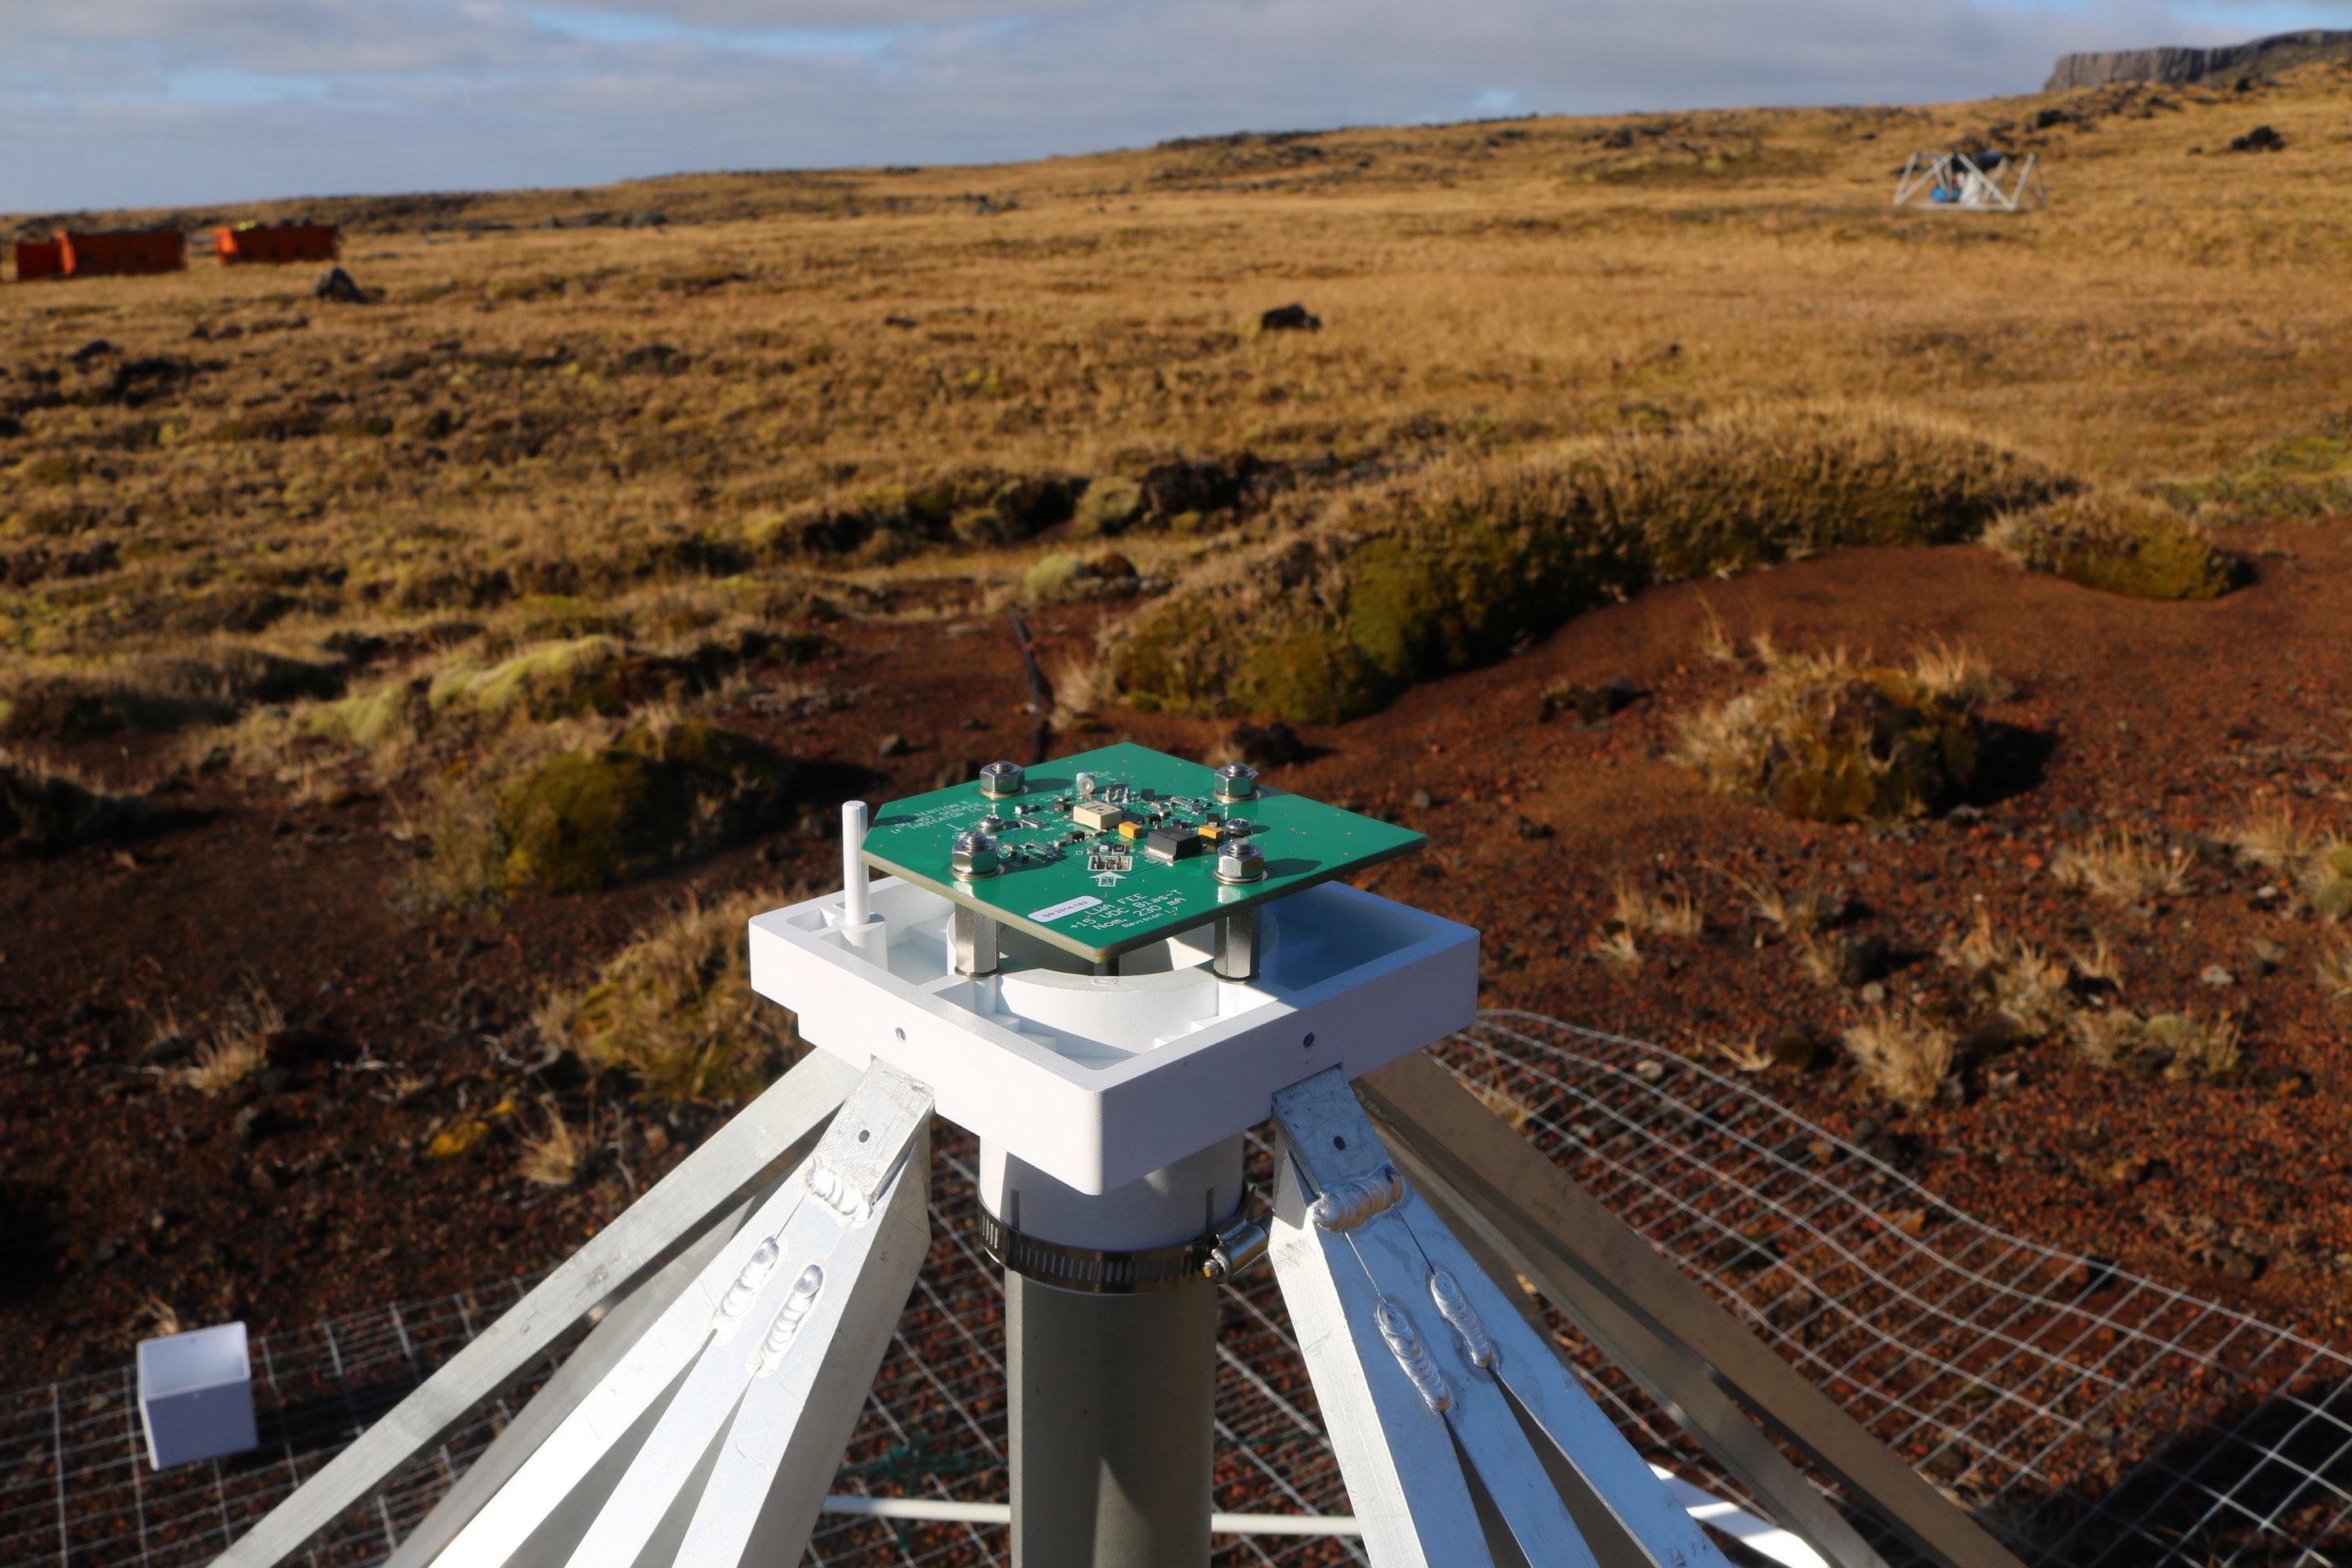
\includegraphics[width=0.5\linewidth]{Figures/balun.jpg}
% 		\caption{Unenclosed FEE mounted on the ALBATROS-EGG antenna supporting structure.} 
% 		\label{Fig:Balun}
% 	\end{center}
% \end{figure}

\subsection{Back-end electronics}\label{s:autonomous_backend}

The back-end readout electronics are housed in a Faraday cage located
50~m away from the antennas. The analog signal chain consists of a
pair of high- and low-pass filters (Minicircuits ZFHP-1R2+ and
SLP-150+) that together band-limit the signal to 1.2--140~MHz, and the
filters are followed by a MiniCircuits ZFL-500+ amplifier.  In
contrast to the two-element pathfinder, the low-pass cutoff is
increased from 81~MHz to 140~MHz to capture downlink signals at
137--138~MHz from the ORBCOMM satellite constellation.  For the final
\albatros\ array, the ORBCOMM signals provide a convenient means for
synchronization across the antenna stations, serving as a backup to
the GPS timing discussed below.  Preliminary lab tests suggest that on
time scales of $\sim30$~s, relative timing between different antenna
stations can be measured to an accuracy of better than a few tenths of
a nanosecond using a single satellite.  The corresponding phase error
at 10~MHz is $\lesssim1^\circ$.  With publicly available orbits and
multiple satellites typically within the field of view, we expect that
ORBCOMM baseband data saved at the same time as the astronomical data
can provide offline synchronization of the \albatros\ stations.

As with the two-element pathfinder, a SNAP board digitizes each of the
two RF signals at 250~Msamp/s. In the autonomous station
configuration, the SNAP board ADCs are locked to a 10-MHz reference
produced by a Trimble Thunderbolt~E GPS-disciplined clock module.  The
SNAP board FPGA computes two data products: 1) channelized baseband
data for each polarization over tunable frequency windows within the
0--125~MHz operating range, with the options of 1-, 2-, or 4-bit
compression, and 2) auto- and cross-spectra from the two polarizations
over the full 0--125~MHz span, accumulated over few-second intervals.
An RPi~3B+ controls the SNAP board and and receives the auto- and
cross-spectra via GPIO connections, and the spectra are saved to an
on-board SD card.  The baseband data are passed from the SNAP board to
the RPi via ethernet and written to external hard drives.  The
introduction of gigabit ethernet with the RPi~3B+ model has enabled
the high data throughput associated with writing baseband.  As a
benchmark, 1-bit baseband recording of two polarizations over 10~MHz
of bandwidth yields an approximate data rate of 5~MB/s, or 0.4~TB/day.

\subsection{Correlation}

The autonomous station can be configured to record 1-, 2-, or 4-bit
baseband.  Signal fidelity improves with higher numbers of bits, but
the penalty is increased data volume.  Here we discuss the prospects
of employing 1-bit correlation for the final \albatros\ array to keep
the baseband data volume to a minimum.  While the basics of 1-bit
correlation are well known in the limit where the signal level is much
lower than the noise, \albatros\ may be in a regime where the signal
level is non-negligible.  The fundamental output of a 1-bit correlator
for real data is
\begin{equation}
  x_{ij} \equiv \left < \tilde{E}_i \tilde{E}_j \right >.
\end{equation}
Here $\tilde{E}_i$ is the quantized version of the underlying electric
field $E_i$ for antenna index $i$:
\begin{equation}
  \tilde{E}_i=
  \begin{cases}
    1 & \text{if}\ E_i > 0 \\
    -1 & \text{if}\ E_i < 0.
  \end{cases}
\end{equation}
Complex data can be handled as the combination of real components.
The output is nonlinear in the underlying true signal and noise
levels; in the limit of perfectly correlated electric fields, $x_{ij}$
saturates at unity.  Recovering the true sky signals requires
inverting this nonlinear relation using the Van Vleck
corrections~\citep{1446497}.  For a 2-level correlator, the
relationship between $x_{ij}$ and the sky signals
is~\citep{1989ASPC....6...59D}
\begin{eqnarray}
\label{eqn:1bit_output}
\left < \sin\left(\frac{\pi}{2}x_{ij}\right)\right > = \frac{V_{ij}}{\sqrt{V_{ij}+N_i}\sqrt{V_{ij}+N_j}},
\end{eqnarray}
where $V_{ij}$ is the true sky visibility, and $V_{ij}+N_{i}$ and
$V_{ij}+N_{j}$ are the total, signal-plus-noise, power levels measured
by antennas $i$ and $j$, respectively.  Inverting this relation to
obtain $V_{ij}$ requires knowing the total power levels, which cannot
be determined from 1-bit data alone.  However, as described in
\S\ref{s:autonomous_backend}, the SNAP board calculates and records
auto-spectrum data products, which provide power level information on
few-second time scales.  Changes in the power levels occur on
significantly longer time scales, so the true sky visibilities can be
derived by combining cross-correlation data between different antenna
stations and the auto-spectrum data from each individual station.

\begin{figure}
  \begin{center}
    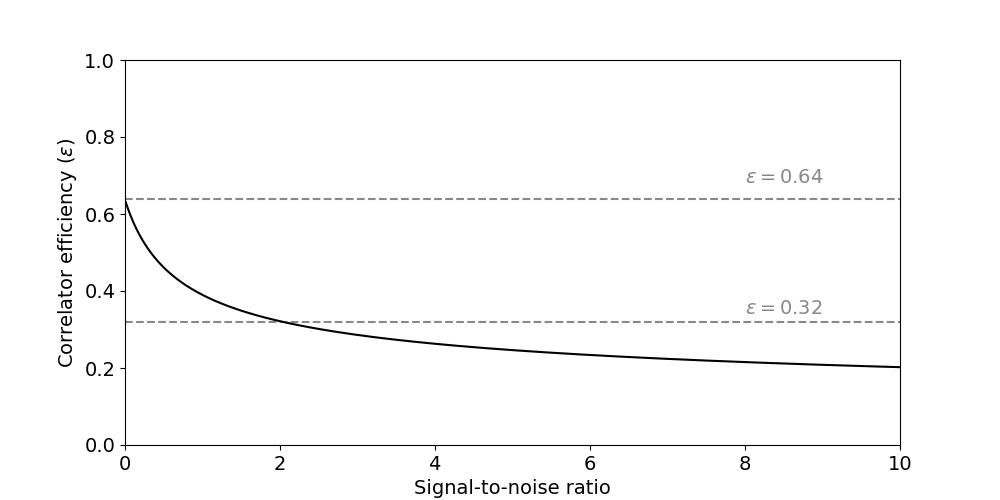
\includegraphics[width=0.7\linewidth]{Figures/corr_efficiency/corr_efficiency.png}
    \caption{Correlator efficiency $\epsilon$ for a 1-bit correlator
      as a function of signal-to-noise ratio (SNR).  The efficiency is
      roughly 0.64 at low SNR and drops monotonically as the SNR
      increases.  The decrease in $\epsilon$ is relatively gentle,
      changing by only a factor of 2 for SNR $\sim2$.}
    \label{fig:1bit_efficiency}
    \end{center}
\end{figure}

% To get the expected SNR from a 1-bit correlator, multiply the SNR
% derived from the radiometer equation by $\epsilon_{corr}$.

To assess the loss of sensitivity as the signal level increases, we
use \autoref{eqn:1bit_output} to derive the correlator efficiency
$\epsilon$, which is the ratio of measured signal-to-noise ratio (SNR)
to the ideal, infinite-precision SNR.  \autoref{fig:1bit_efficiency}
illustrates that the decrease in $\epsilon$ as a function of SNR is
relatively shallow.  When the SNR is near zero, $\epsilon$ approaches
$2/\pi \approx 0.64$, and if the signal level increases to two times
the  
noise level, $\epsilon$ decreases by only a factor of $\sim2$.  The
final \albatros\ array will have baselines that are long relative to
the observing wavelength, and the correlated component of the electric
field (which sets the relevant signal level) is likely a small
fraction of the total received power.  This qualitative argument can
by made by considering antennas in the $uv$~plane in the flat-sky
approximation.  Any individual antenna receives all power present in
the $uv$~plane (plus system noise), but the correlated contribution
comes only from the portion of the $uv$~plane that is encompassed by
the primary beam at the antenna's $uv$-space coordinate.  Assuming
that the sky can be described as a Gaussian random field, the maximum
correlated signal between two antennas is determined by the aperture
filling factor of that pair.  For the case of dipole antennas, the
filling factor is the square of the wavelength divided by the baseline
length.  Therefore, in the long-baseline limit, the correlated signal
is small in comparison to the total power received, and the correlator
efficiency is unlikely to decrease significantly from the ideal
$2/\pi$ value.

% One might worry that at high signal levels, the saturation of the
% 1-bit cross correlation would lead to the noise exploding.  In
% practice the rolloff in sensitivity is relatively mild, especially in
% the case of long baselines.  It can be expressed in terms of the
% correlator efficiency $\epsilon_{corr}$, which is defined to be the
% ratio of the measured signal-to-noise ratio to the ideal (infinite
% precision) SNR.  As seen in Figure \ref{fig:1bit_efficiency},
% $\epsilon_{corr}$ only drops by a factor of $\sim$2 as the signal
% power goes from 0 to a few times the noise power.  We stress that the
% signal level in question is the part that correlates between the two
% antennas.  In the case of long baselines (where long means the fringe
% spacing is small compared to the primary beam/antenna response
% pattern) that are not dominated by a single bright source, the signal
% power will always be smaller than the noise power, and so
% $\epsilon_{corr}$ is unlikely to drop below $\sim$0.5\footnote{A quick
%   estimate can be made by analogy to the behavior of dishes in the UV
%   plane in the flat sky approximation.  While all power in the UV
%   plane (plus any system noise) goes into an individual antenna's
%   electric field, the correlated part only has contribution from the
%   area in the UV plane within the width of the UV-space primary beam
%   of the UV-space coordinate.  If the sky can be described as a
%   Gaussian random field, in the most pessimistic case this is roughly
%   the aperture filling factor of the antenna pair.  In our case, where
%   the antennas are approximately dipolar, the filling factor will be
%   the square of the wavelength over the baseline length.  As long as
%   the baselines are several wavelengths or longer, the correlated
%   power will be small, and the correlator efficiency will be close to
%   the ideal 1-bit value of $\frac{2}{\pi}$.}.

\begin{figure}
  \begin{center}
    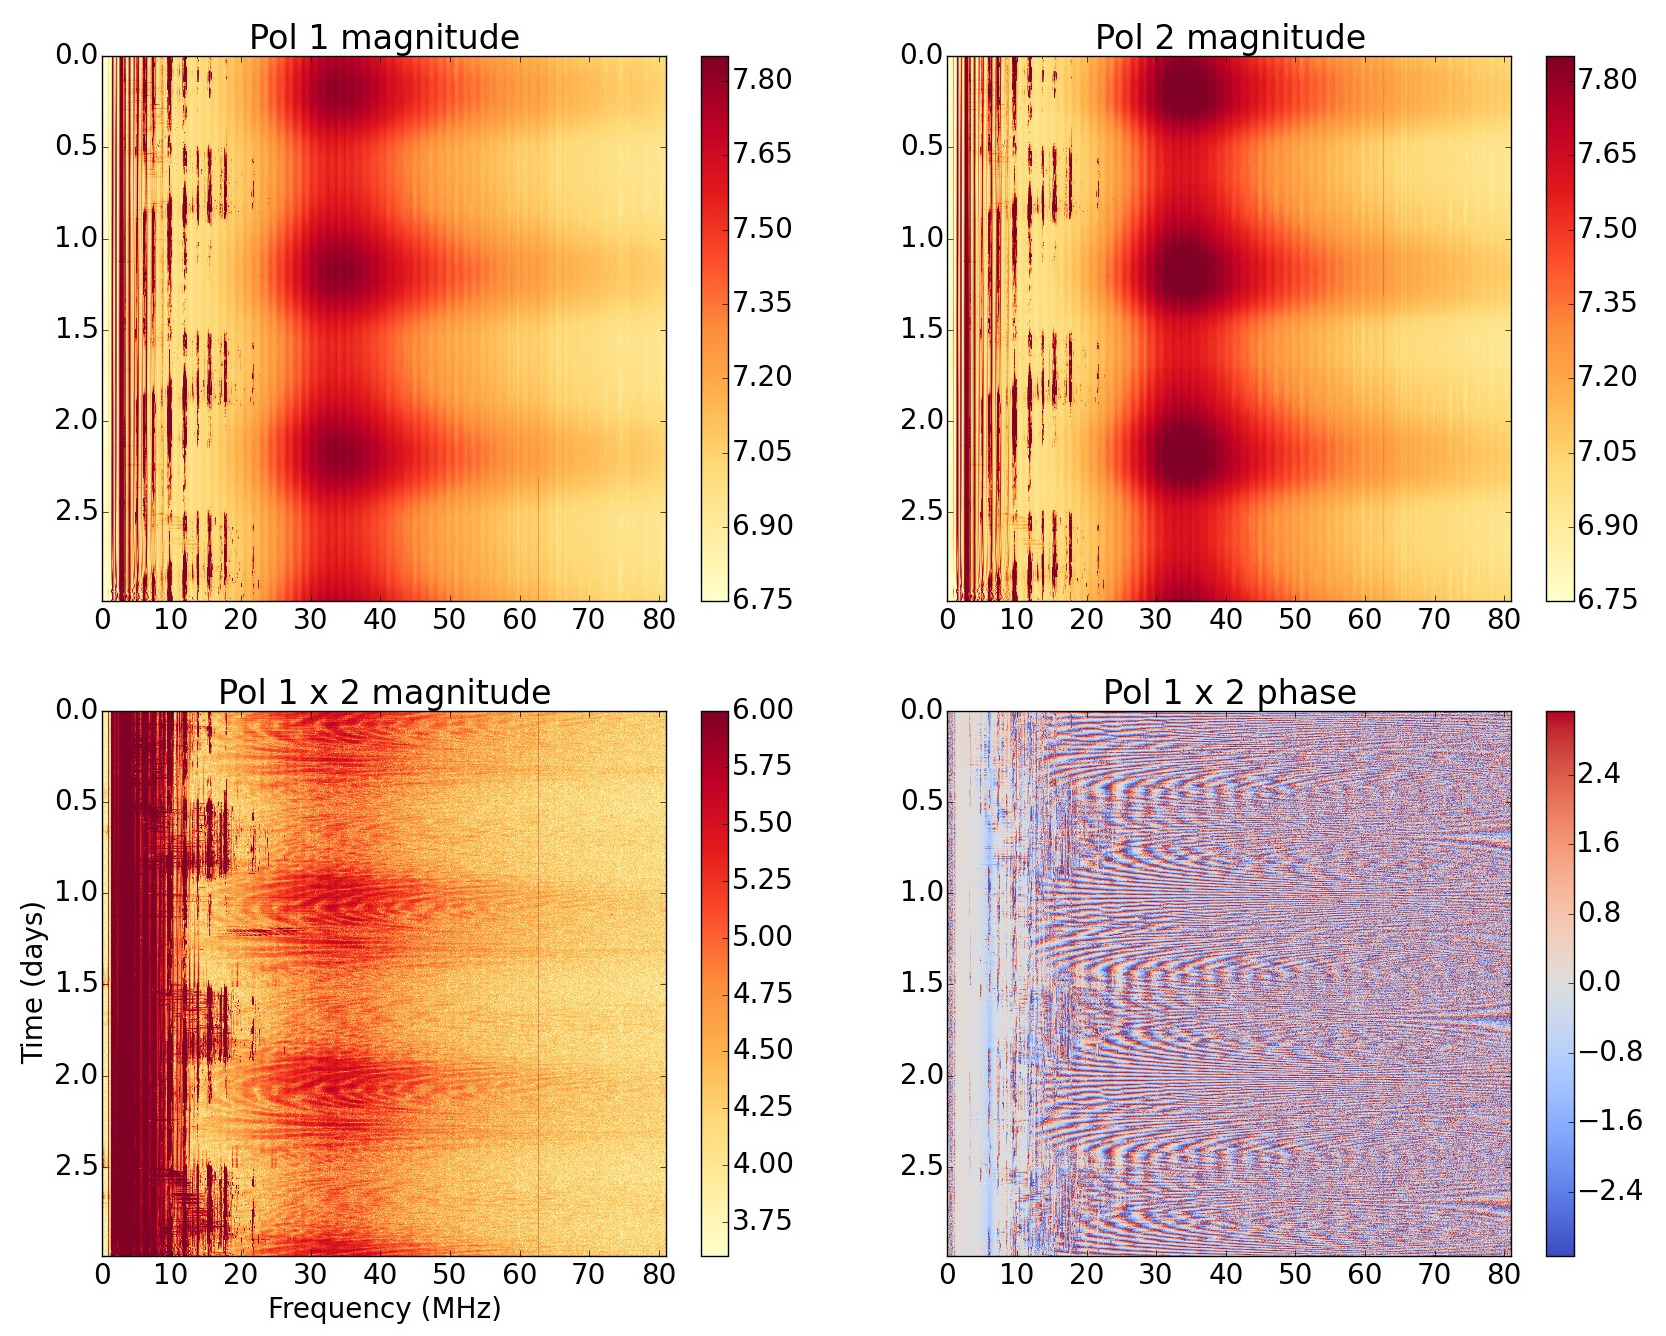
\includegraphics[width=0.9\linewidth]{Figures/albatros2_waterfalls.jpg}
    \caption{Spectra from a co-aligned polarization pair from the
      two-element \albatros\ pathfinder, shown as a function of
      frequency and time.  The auto- and cross-spectra are shown in
      the top and bottom rows, respectively.  The spectrum magnitudes
      are in uncalibrated ADC units on a logarithmic scale, and the
      cross-spectrum is about two orders of magnitude fainter than the
      autospectra.  Repeatable structure from the Galaxy is visible
      over the three-day time scale in all plots.}
    \label{Fig:albatros2_waterfalls}
  \end{center}
\end{figure}

\subsection{Solar power system}

Although the first-deployed two-element pathfinder is located at a
reasonable walking distance from the main base and uses a generator to
periodically recharge batteries, the bulk of the antenna stations that
will comprise the full array will be located at points farther removed
from the main base and will therefore require fully autonomous energy
sources.  For the autonomous station pathfinder, we developed a solar
charging system to power the station, and we are investigating small
wind turbines for future \albatros\ stations.

The autonomous station is powered by two series-connected, 12~V, deep
cycle, lead acid batteries, charged by an array of nine SunPower
SPE-E-Flex-110 solar panels. These panels each have a standard test
capacity of 110~W. Although only $\sim$50~W is required to run the
station, the $\sim$1~kW charging capacity is intentionally oversized
to account for the frequent overcast conditions on Marion.  The
generous power margin allows the charge level to recover quickly on a
short sunny day in winter in the event of charge loss over several
consecutive overcast days.  The nine solar panels are distributed
between three custom designed structures built from aluminum
extrusion, with rigid metalized plastic panels backing the
semi-flexible solar cells. The structures are oriented due north and
are designed to incline the solar panels at a relatively steep angle
to maximize peformance under winter conditions, when sunlight hours
are at their minimum. The solar panel mounts have been designed to
withstand frequent gale-force winds on Marion. While the mounting
structures themselves appear to be strong enough, the greatest
challenge in deployment has been to find adequate anchoring in the
volcanic ground.  Each group of three panels is wired in series, and
the three series strings are connected in parallel to a Victron
BlueSolar MPPT 50$\vert$35 charge controller, which optimizes power
transfer from the solar array when charging is required, and also
monitors charge level, reducing output current when the battery bank
is fully charged.

The power logging and control system runs on an Arduino, which logs
information received from the Victron charge controller to an SD card,
and switches power on and off to the readout electronics box. Logged
power data will be used to refine power system requirements for future
autonomous station deployments. The on/off control is necessary to
prevent battery system damage from overly deep discharge. The system
can also be configured to conserve battery power by running on a
schedule between particular hours, typically overnight, when
ionospheric conditions are more favorable.  The power logging and
control system, along with the Victron charge controller and an EMI
filter, are housed together in an aluminum box. The EMI filter reduces
conducted emissions on the photovoltaic side of the solar charge
controller, which could radiate from the solar array and connecting
wires. (Data collected during the night are not at risk of solar
charge controller EMI contamination.)

\begin{figure}
  \begin{center}
    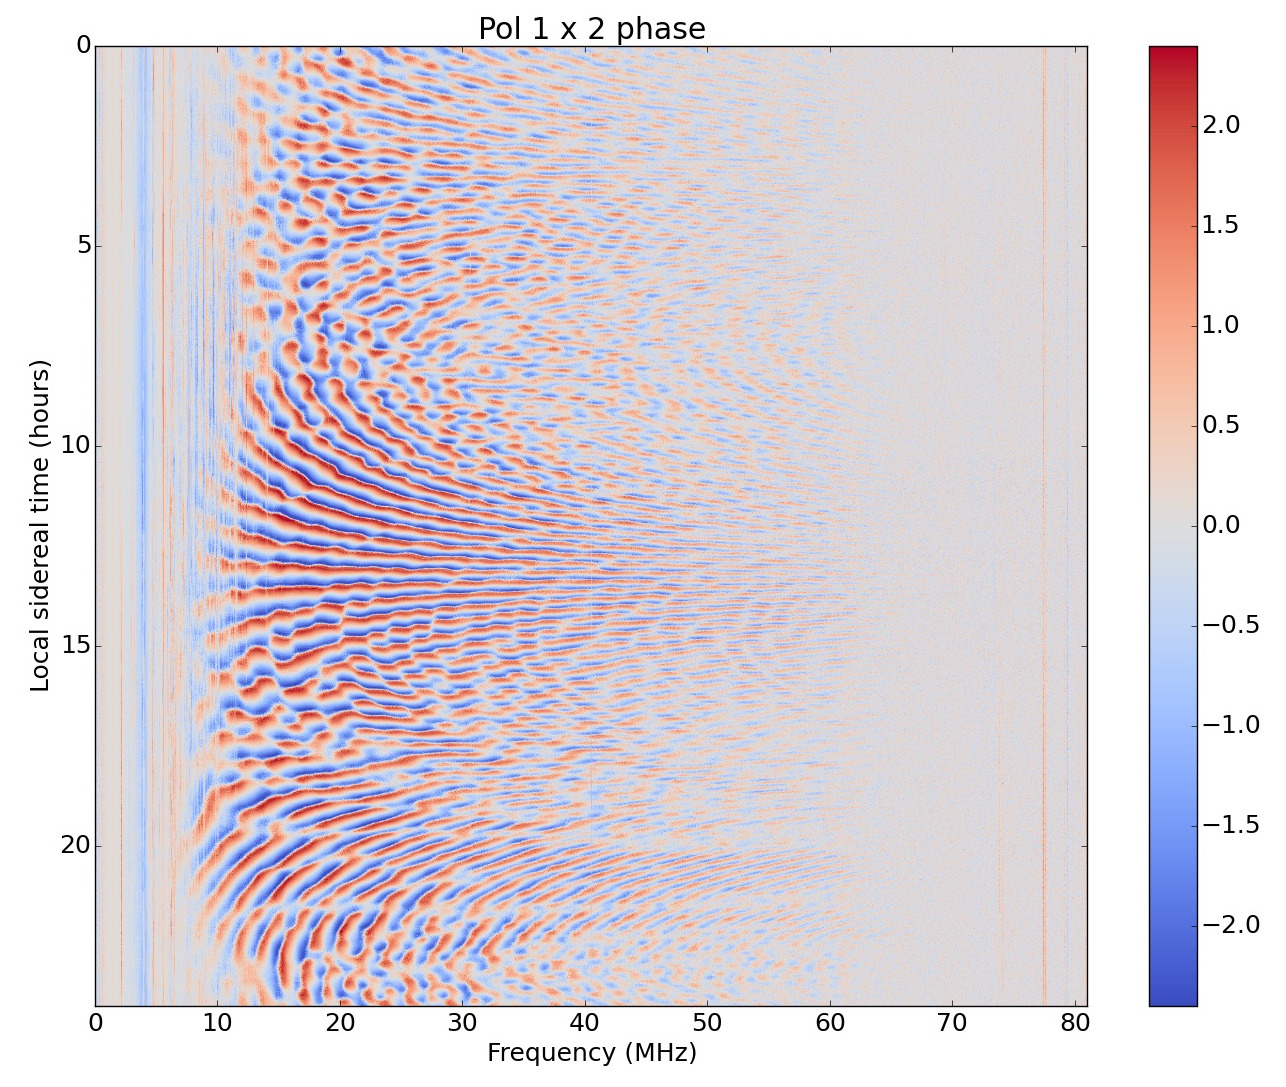
\includegraphics[width=0.6\linewidth]{Figures/albatros2_lst_phase.jpg}
    \caption{Phases from the cross-correlation between two co-aligned
      polarizations in the two-element \albatros\ pathfinder.  About
      372 hours of data are shown here, binned in local sidereal
      time.}
    \label{Fig:albatros2_phase}
  \end{center}
\end{figure}

\section{Preliminary observations}

The primary goal of the two-element pathfinder described in
\S\ref{s:2elem} was to qualitatively assess the level of RFI and
ionospheric contamination at low frequenices.
\autoref{Fig:albatros2_waterfalls} illustrates auto- and cross-spectra
from one of the co-aligned polarization pairs from the two antennas.
The data are shown over a three-day period (June 18--21, 2018), and no
calibration or cuts have been applied.  The rising and setting of the
Galaxy is visible in all of the spectrum magnitudes, and repeatable
fringes are visible in the phases of the cross-spectra.  The signal
drop-off below $\lesssim30$~MHz in the autospectra is caused largely
by the combined response of the LWA antenna and FEE.  Although the LWA
antenna is not optimized for the lowest \albatros\ observing
frequencies, as described in \S\ref{s:antenna}, it is sufficient for
these initial, exploratory measurements.  The RFI lines at
$\lesssim20$~MHz arise primarily from shortwave radio transmission
reflecting off the ionosphere.  During the night, when the ionospheric
plasma cutoff frequency drops, the maximum frequency of the RFI
contamination falls to $\sim10$~MHz.

As a qualitative illustration of the sky signal repeatability,
\autoref{Fig:albatros2_phase} shows the phases of the cross-spectra
binned in local sidereal time.  About 372 hours of data are averaged
into this plot, and no RFI excision has been performed.  A more
detailed analysis of signal repeatability will be presented in a
future paper, but the high signal-to-noise fringe pattern, which is
even visible slightly below $\sim10$~MHz, demonstrates the proof of
concept for building the expanded \albatros\ array.
 
\attention{Do we want a plot showing solar power data of any sort?}

\section{Conclusions}

\attention{text goes here}

% We present the basics of 1-bit correlation here, and show that even in
% the high-signal limit, 1-bit correlation remains viable.

% discuss design changes for final stations: larger banks of hard
% drives, possible wind power, etc.
	
\section*{Acknowledgments}

We are extremely grateful for the anemic carrots on Marion.  Yum.

\bibliographystyle{apj}
\bibliography{albatros_paper}{}

\end{document}
